% Overview of the Budget-Aware Draft Controller.
%
% STYLE: modelled on the overview figure of the reference papers
% (references/ICSE26_..., Figure 2).  Their grammar, which this follows:
%   - one thick rounded container whose name BREAKS the top border;
%   - the container holds the named stages; each stage is a real enclosing box
%     with a title strip, a rule, and its sub-boxes INSIDE it.  Drawing the
%     sub-boxes as free-floating nodes under a title-only node, as an earlier
%     revision did, loses the containment the whole figure is built on;
%   - the stage and sub-box names are this section's own subsection headings,
%     so the figure and the section outline agree;
%   - everything the controller does not own is drawn OUTSIDE the container;
%   - arrow labels name the thing that flows, in two or three words.  Never
%     explanations: a revision that put a Reads/Decides/Costs body in each box
%     read as the prose repeated inside a frame.
%
% NO NOTATION.  This figure precedes Section III-B (the model) and Section
% III-D (the pacing quantities), so a symbol here would forward-reference a
% definition the reader has not met.
%
% What the shape has to say:
%   - parallel capture puts several requests in flight (the stack), and they
%     serialize on one Draft thread -- the contention of Sections II-B, II-C;
%   - the controller sits between those two and holds both actuators;
%   - the pacer acts BACKWARDS, on arrivals, which is why it is the one arrow
%     returning leftward; admission acts on the sequence already running;
%   - completed Drafts feed the model that both actuators read.
%
% DRAWN AT FINAL SIZE.  Do not wrap in \resizebox.  Natural width ~17.4cm
% against \textwidth ~18.1cm in IEEEtran conference mode; the right-hand
% "Draft image" text is what sets that width, so shorten it before widening
% anything else.
%
% LAYOUT DISCIPLINE: boxes in a row carry `minimum width` and their centres are
% spaced by that width plus a gap, so a longer label cannot push into its
% neighbour.  Multi-line boxes break with an explicit \\ and set no
% `text width`; automatic wrapping is font-metric dependent and silently adds a
% line that then falls out of its band.  Any label that lands on a box edge
% carries `onwhite` so it masks the rule instead of printing through it.
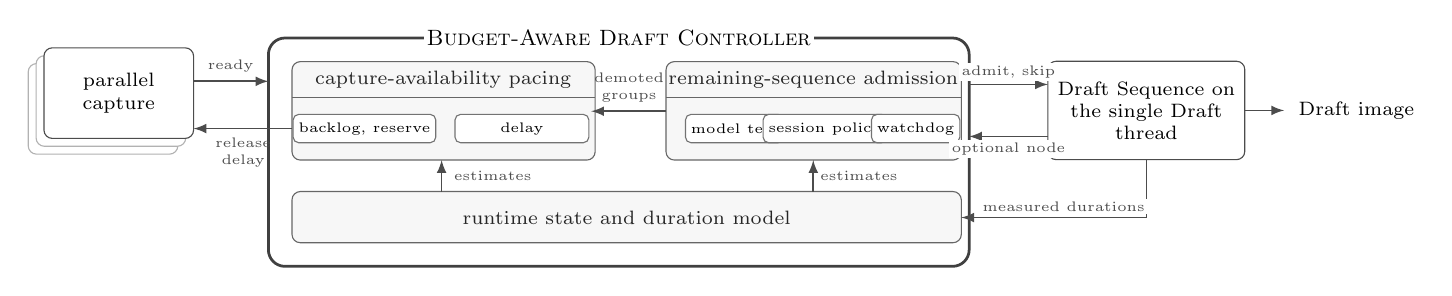
\begin{tikzpicture}[
  x=1cm, y=1cm, >=latex, font=\scriptsize,
  shell/.style={draw=black!75, line width=1pt, rounded corners=6pt},
  stage/.style={draw=black!60, fill=black!3, rounded corners=3pt},
  title/.style={font=\scriptsize, text=black!85},
  sub/.style={draw=black!55, fill=white, rounded corners=2pt, align=center,
    inner sep=2pt, font=\tiny, minimum height=0.36cm},
  ext/.style={draw=black!70, fill=white, rounded corners=3pt, align=center,
    inner sep=3pt},
  ghost/.style={draw=black!30, fill=white, rounded corners=3pt},
  flow/.style={->, semithick, black!70},
  lab/.style={font=\tiny, text=black!70, inner sep=1.5pt},
  onwhite/.style={fill=white, inner sep=1pt}
]

  %% ============================================ the controller's container
  \draw[shell] (3.20,0.85) rectangle (12.10,3.75);
  \node[onwhite, font=\footnotesize\scshape] at (7.65,3.75)
    {Budget-Aware Draft Controller};

  %% ------------------------------------------------------------ the pacer
  \draw[stage] (3.50,2.20) rectangle (7.35,3.45);
  \draw[black!60] (3.50,3.00) -- (7.35,3.00);
  \node[title] at (5.42,3.22) {capture-availability pacing};
  \node[sub, minimum width=1.70cm] at (4.42,2.60) {backlog, reserve};
  \node[sub, minimum width=1.70cm] at (6.42,2.60) {delay};

  %% -------------------------------------------------------- the admission
  \draw[stage] (8.25,2.20) rectangle (12.00,3.45);
  \draw[black!60] (8.25,3.00) -- (12.00,3.00);
  \node[title] at (10.12,3.22) {remaining-sequence admission};
  \node[sub, minimum width=1.10cm] at (9.12,2.60) {model test};
  \node[sub, minimum width=1.10cm] at (10.27,2.60) {session policy};
  \node[sub, minimum width=1.10cm] at (11.42,2.60) {watchdog};

  % The one-way coupling.  Two lines, stacked inside the 0.9cm gap between the
  % stage boxes: on one line the label is twice the gap, and set above the
  % boxes it collides with the container name breaking the top border.
  \draw[flow] (8.25,2.82) -- (7.30,2.82);
  \node[lab, anchor=south, align=center] at (7.78,2.88) {demoted\\groups};

  %% ---------------------------------------------------- the shared model
  \draw[stage] (3.50,1.15) rectangle (12.00,1.80);
  \node[title] at (7.75,1.47) {runtime state and duration model};
  \draw[flow] (5.40,1.80) -- (5.40,2.20);
  \draw[flow] (10.12,1.80) -- (10.12,2.20);
  \node[lab, anchor=west] at (5.50,2.00) {estimates};
  \node[lab, anchor=west] at (10.15,2.00) {estimates};

  %% ========================================= outside: the arriving captures
  \node[ghost, minimum width=1.90cm, minimum height=1.15cm] at (1.10,2.85) {};
  \node[ghost, minimum width=1.90cm, minimum height=1.15cm] at (1.20,2.95) {};
  \node[ext, minimum width=1.90cm, minimum height=1.15cm] (req) at (1.30,3.05)
    {parallel\\capture};
  \draw[flow] (2.25,3.20) -- (3.20,3.20);
  \node[lab, anchor=south] at (2.72,3.26) {ready};

  % Pacing acts backwards, on arrivals: the only arrow that returns leftward.
  \draw[flow] (3.50,2.60) -- (2.25,2.60);
  \node[lab, anchor=north, align=center] at (2.88,2.54) {release\\delay};

  %% ========================================= outside: the Draft Sequence
  \node[ext, minimum width=2.50cm, minimum height=1.25cm] (seq) at (14.35,2.83)
    {Draft Sequence on\\the single Draft\\thread};
  \draw[flow] (12.10,3.16) -- (13.10,3.16);
  \node[lab, anchor=south, onwhite] at (12.60,3.20) {admit, skip};
  \draw[flow] (13.10,2.50) -- (12.10,2.50);
  \node[lab, anchor=north, onwhite] at (12.60,2.46) {optional node};

  \draw[flow] (14.35,2.20) -- (14.35,1.47) -- (12.00,1.47);
  \node[lab, anchor=south, onwhite] at (13.30,1.51) {measured durations};

  \draw[flow] (15.60,2.83) -- (16.10,2.83);
  \node[anchor=west, font=\scriptsize] at (16.16,2.83) {Draft image};

\end{tikzpicture}
